% (c) 2012-2014 Dimitrios Vrettos - d.vrettos@gmail.com

\chapter{Prodotti notevoli}

Con l'espressione \emph{prodotti notevoli} si indicano alcune
identità che si ottengono in seguito alla moltiplicazione di polinomi
aventi caratteristiche particolari facili da ricordare.

\section{Quadrato di un binomio}\label{sect:quadrato_di_un_binomio}

Consideriamo il binomio~$A+B$ in cui~$A$ e~$B$ rappresentano due monomi ed
analizziamo che cosa succede moltiplicando il binomio per se
stesso, eseguendo cioè la
moltiplicazione~$\left(A+B\right)\left(A+B\right)$, che sotto forma di potenza si scrive~$\left(A+B\right)^{2}$

\[\left(A+B\right)^{2}=\left(A+B\right)\left(A+B\right)=A^{2}+{AB}+{BA}+B^{2}=A^{2}+2{AB}+B^{2}.\]

Pertanto si può scrivere direttamente~$\left(A+B\right)^{2}=A^{2}+2{AB}+B^{2}$.

Analizzando il prodotto ottenuto si può notare che è costituito da
tre termini ed in particolare due termini sono costituiti dal prodotto
di ciascun monomio per se stesso ed un termine è costituito dal
prodotto dei due monomi moltiplicato a sua volta per~2.

\osservazione Il quadrato di un binomio è
uguale alla somma tra il quadrato del primo termine, il quadrato del
secondo termine e il doppio prodotto del primo termine per il secondo.

Nell'identità precedente, $A$ e~$B$ rappresentano due monomi qualsiasi,
quindi la scrittura~$A+B$ deve intendersi come somma algebrica di due
monomi che, rispetto al segno, possono essere concordi o discordi.

Ne consegue che:

\begin{enumeratea}
\item $A^{2}$ e~$B^{2}$ sono sempre positivi
perché prodotto di fattori uguali e quindi concordi;
\item $2AB$ è positivo se~$A$ e~$B$ sono concordi, negativo se sono
discordi.
\end{enumeratea}

\begin{wrapfloat}{figure}{r}{0pt}
 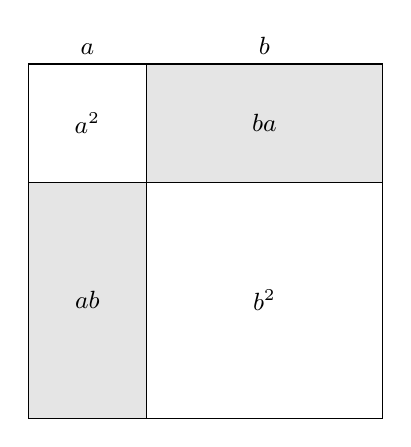
\begin{tikzpicture}[x=5mm, y=5mm,font=\small]
\definecolor{area}{gray}{0.9}
\draw(0,0) rectangle (9,9); 
\begin{scope}[fill=area, draw=black]
\filldraw (0,0) rectangle  (3,6);
\filldraw (3,6) rectangle (9,9);
\end{scope}

\node[above]  at (1.5,9) {$a$};
\node[above]  at (6,9) {$b$};
\node  at (1.5,7.5) {$a^2$};
\node  at (6,7.5) {$ba$};
\node  at (1.5,3) {$ab$};
\node  at (6,3) {$b^2$};	

\end{tikzpicture}
\end{wrapfloat}

È possibile dare anche
un'interpretazione geometrica della formula~$\left(A+B\right)^{2}=A^{2}+2{AB}+B^{2}$,
sostituendo~$A$ e~$B$ rispettivamente con le misure~$a$ e~$b$
di due segmenti.

Prendiamo due segmenti di lunghezza~$a$ e~$b$ e portiamo a
coincidere il secondo estremo del segmento lungo~$a$ con il
primo estremo del segmento di lunghezza~$b$: in questo modo
otteniamo un segmento di lunghezza~$a+b$. Costruiamo il quadrato di
lato~$a+b$, il quale avrà area~$(a+b)^{2}$ e dividiamolo come
nella figura a fianco.

Puoi notare che il quadrato di lato~$a+b$ è composto da due quadrati
di area rispettivamente~$a^{2}$ e~$b^{2}$ e
da due rettangoli di area~$ab$. Di conseguenza
l'area del quadrato è uguale a:~$(a+b)^{2}=a^{2}+b^{2}+{ab}+{ab}=a^{2}+b^{2}+2{ab}$.

\vspazio\ovalbox{\risolvii \ref{ese:12.1}, \ref{ese:12.2}, \ref{ese:12.3}, \ref{ese:12.4}, \ref{ese:12.5}, \ref{ese:12.6}, \ref{ese:12.7}, \ref{ese:12.8}, \ref{ese:12.9}, \ref{ese:12.10}}

\section{Quadrato di un polinomio}\label{sect:quadrato_di_un_polinomio}

Si consideri il trinomio~$A+B+C$, il suo quadrato sarà dato da:
\begin{align*}
\left(A+B+C\right)^{2}&=\left(A+B+C\right)\left(A+B+C\right)\\
&=A^{2}+{AB}+{AC}+{BA}+B^{2}+{BC}+{CA}+{CB}+C^{2}\\
&=A^{2}+B^{2}+C^{2}+2{AB}+2{AC}+2{BC}.
\end{align*}

Pertanto si può scrivere $\left(A+B+C\right)^{2}=A^{2}+B^{2}+C^{2}+2{AB}+2{AC}+2{BC}$.

\osservazione Il quadrato di un polinomio è uguale alla somma
dei quadrati dei monomi che lo compongono e dei doppi prodotti di ogni
termine per ciascuno dei successivi.

Nel caso di un polinomio composto da quattro monomi si ha:
%\[\left(x+y+z+t\right)^{2}=x^{2}+y^{2}+z^{2}+t^{2}+2{xy}+2{xz}+2{xt}+2{yz}+2{yt}+2{zt}.\]
\[\left(A+B+C+D\right)^{2}=A^{2}+B^{2}+C^{2}+D^{2}+2{AB}+2{AC}+2{AD}+2{BC}+2{BD}+2{CD}.\]

\ovalbox{\risolvii \ref{ese:12.11}, \ref{ese:12.12}, \ref{ese:12.13}, \ref{ese:12.14}, \ref{ese:12.15}}

\section{Prodotto della somma di monomi per la loro differenza}\label{sect:differenza_di_quadrati}

Si consideri il seguente prodotto:

\begin{equation}\label{eq:prodmon}
 \left(A+B\right)\left(A-B\right)=A^{2}-{AB}+{AB}-B^{2}=A^{2}-B^{2}.
\end{equation}

Pertanto, quando eseguiamo il prodotto tra due binomi che hanno due
termini uguali e due termini opposti i prodotti incrociati si annullano
e rimangono i due prodotti del termine uguale per se stesso e dei due
termini opposti, il primo prodotto risulterà sempre positivo, il
secondo prodotto risulterà sempre negativo. Quindi si può scrivere
$\left(A+B\right)\left(A-B\right)=A^{2}-B^{2}$.

\osservazione Il prodotto tra due binomi che hanno due termini
uguali e due termini opposti si ottiene semplicemente moltiplicando tra
di loro i due termini uguali e i due termini opposti, ottenendo così una differenza di quadrati.

\begin{exrig}
 \begin{esempio}
$\left(3a^{2}+5{ab}\right)\cdot \left(3a^{2}-5{ab}\right).$

Moltiplichiamo~$3a^{2}\cdot 3a^{2}$ e
$\left(+5{ab}\right)\cdot\left(-5{ab}\right)$, otteniamo
$9a^{2}-25a^{2}b^{2}$.
 \end{esempio}

 \begin{esempio}
 \[\left(-{\frac{1}{4}}x^{2}+b\right)\cdot \left(+{\frac{1}{4}}x^{2}+b\right).\]

Osserviamo che il monomio che cambia di segno è~$\frac{1}{4}x^{2}$,
nella forma generale \eqref{eq:prodmon} occorre porre~$A=b$ e $B=\frac{1}{4}x^{2}$.
Il risultato è quindi~$A^{2}-B^{2}=b^{2}-\frac{1}{16}x^{4}$.
 \end{esempio}

 \begin{esempio}
 Senza utilizzare la calcolatrice, calcola mentalmente il prodotto~$28\cdot 32$.

Svolgimento:~$28\cdot 32=(30-2)\cdot(30+2)=900-4=896$.
 \end{esempio}

 \begin{esempio}
$(2x+1-y)(2x+1+y).$

Possiamo riscrivere il prodotto nella forma
\[\big((\underbrace{2x+1}_{A})-\underbrace{y}_{B}\big)\big((\underbrace{2x+1}_{A})+\underbrace{y}_{B}\big)=\underbrace{(2x+1)^{2}}_{A^{2}}-\underbrace{y^{2}}_{B^{2}}=4x^{2}+4x+1-y^{2}.\]
 \end{esempio}

\end{exrig}

\ovalbox{\risolvii \ref{ese:12.16}, \ref{ese:12.17}, \ref{ese:12.18}, \ref{ese:12.19}, \ref{ese:12.20}, \ref{ese:12.21}, \ref{ese:12.22}, \ref{ese:12.23}}

\section{Cubo di un binomio}\label{sect:cubo_di_un_binomio}

Si consideri il binomio~$A+B$, il suo cubo sarà dato da:

\begin{align*}
\left(A+B\right)^{3}&=\left(A+B\right)^{2}\left(A+B\right)=\left(A^{2}+2{AB}+B^{2}\right)\left(A+B\right)\\
%\left(A+B\right)^{3}&=\left(A+B\right)^{2}\left(A+B\right)\\
%&=\left(A^{2}+2{AB}+B^{2}\right)\left(A+B\right)\\
&=A^{3}+A^{2}B+2A^{2}B+2{AB}^{2}+{AB}^{2}+B^{3}\\
&=A^{3}+3A^{2}B+3{AB}^{2}+B^{3}.
\end{align*}

Pertanto si può scrivere
$\left(A+B\right)^{3}=A^{3}+3A^{2}B+3{AB}^{2}+B^{3}$.

\osservazione Il cubo di un binomio è uguale alla somma tra il
cubo del primo monomio, il triplo prodotto del quadrato del primo
monomio per il secondo, il triplo prodotto del quadrato del secondo
monomio per il primo e il cubo del secondo monomio.

Essendo~$\left(A-B\right)^{3}=\left[A+\left(-B\right)\right]^{3}$, il
cubo della differenza di due monomi si ottiene facilmente dal cubo
della somma, quindi
$\left(A-B\right)^{3}=A^{3}-3A^{2}B+3{AB}^{2}-B^{3}$.

\vspazio\ovalbox{\risolvii \ref{ese:12.24}, \ref{ese:12.25}, \ref{ese:12.26}, \ref{ese:12.27}}

\section{Potenza n-esima di un binomio}

Finora abbiamo calcolato le potenze del binomio~$a+b$ fino
all'ordine 3, in questo paragrafo ci si propone di
fornire un criterio che permetta di calcolare la potenza~$(a+b)^{n}$,
con~$n\in \insN$. Osserviamo le potenze ottenute:
\begin{multline*}
\\(A+B)^{0}=1\\
(A+B)^{1}=A+B\\
(A+B)^{2}=A^{2}+2AB+B^{2}\\
(A+B)^{3}=A^{3}+3A^{2}B+3AB^{2}+B^{3}.\\
\end{multline*}
Si può notare che:

\begin{itemize*}
\item lo sviluppo di ciascuna potenza dà origine a un polinomio
omogeneo dello stesso grado dell'esponente della
potenza, completo e ordinato secondo le potenze decrescenti di~$A$ e crescenti di~$B$;
\item il primo coefficiente è sempre uguale a~1;
\item i coefficienti di ciascuna riga si ottengono utilizzando una
disposizione dei numeri a triangolo, detto \emph{triangolo di Tartaglia}.
\end{itemize*}

\begin{center}
 \begin{tikzpicture}[x=9mm,y=5mm]

  \tikzset{box/.style={
      minimum height=5mm,
      inner sep=.7mm,
      outer sep=0mm,
      text width=10mm,
      text centered,
      font=\small\ttfamily,
      line width=.25mm,
   }
} 
 \node[box=odd] (p-0-0) at (0,0) {1};
  \foreach \linea in {1,...,6} {
    \node[box=odd] (p-\linea-0) at (-\linea/2,-\linea) {1};
    \pgfmathsetmacro{\valore}{1};
    \foreach \col in {1,...,\linea} {
      \pgfmathtruncatemacro{\valore}{\valore*((\linea-\col+1)/\col)+0.5};
      \global\let\valore=\valore
      \coordinate (pos) at (-\linea/2+\col,-\linea);
      \pgfmathtruncatemacro{\rest}{mod(\valore,2)}
      \ifnum \rest=0
        \node[box=even] (p-\linea-\col) at (pos) {\valore};
      \else
        \node[box=odd] (p-\linea-\col) at (pos) {\valore};
      \fi
    }
  }
\end{tikzpicture}
\end{center}

In questo triangolo i numeri di ciascuna riga (tranne il primo e
l'ultimo che sono uguali a~1) sono la somma dei due
soprastanti della riga precedente. Nella figura che segue evidenziamo
come costruire il triangolo:

\begin{center}
\begin{tikzpicture}[x=12mm,y=8mm]
  \tikzset{
    box/.style={
      minimum height=5mm,
      inner sep=.7mm,
      outer sep=0mm,
      text width=10mm,
      text centered,
      font=\small\ttfamily,
      line width=.25mm,
    },
    link/.style={->,blue,line width=.3mm},
    plus/.style={text=red,font=\small\ttfamily}
  }
 
  \node[box=odd] (p-0-0) at (0,0) {1};
  \foreach \linea in {1,...,4} {
    \node[box=odd] (p-\linea-0) at (-\linea/2,-\linea) {1};
    \pgfmathsetmacro{\valore}{1};
    \foreach \col in {1,...,\linea} {
      \pgfmathtruncatemacro{\valore}{\valore*((\linea-\col+1)/\col)+0.5};
      \global\let\valore=\valore
      \coordinate (pos) at (-\linea/2+\col,-\linea);
      \pgfmathtruncatemacro{\rest}{mod(\valore,2)}
      \ifnum \rest=0
        \node[box=even] (p-\linea-\col) at (pos) {\valore};
      \else
        \node[box=odd] (p-\linea-\col) at (pos) {\valore};
      \fi
      \ifnum \col<\linea
        \node[plus,above=0mm of p-\linea-\col]{+};
        \pgfmathtruncatemacro{\plinea}{\linea-1}
        \pgfmathtruncatemacro{\pcol}{\col-1}
        \draw[link] (p-\plinea-\pcol) -- (p-\linea-\col);
        \draw[link] ( p-\plinea-\col) -- (p-\linea-\col);
      \fi
    }
  }
\end{tikzpicture}
\end{center}


Con questa semplice regola si hanno gli sviluppi:

\begin{itemize*}
\item $(A+B)^{0}=1$;
\item $(A+B)^{1}=A+B$;
\item $(A+B)^{2}=A^{2}+2AB+B^{2}$;
\item $(A+B)^{3}=A^{3}+3A^{2}B+3AB^{2}+B^{3}$;
\item $(A+B)^{4}=A^{4}+4A^{3}B+6A^{2}B^{2}+4AB^{3}+B^{4}$;
\item $(A+B)^{5}=A^{5}+5A^{4}B+10A^{3}B^{2}+10A^{2}B^{3}+5AB^{4}+B^{5}$.
\end{itemize*}

\ovalbox{\risolvii \ref{ese:12.28}, \ref{ese:12.29}, \ref{ese:12.30}}
\newpage
% (c) 2012 Claudio Carboncini - claudio.carboncini@gmail.com
% (c) 2012 -2014 Dimitrios Vrettos - d.vrettos@gmail.com

\section{Esercizi}
\subsection{Esercizi dei singoli paragrafi}
\subsubsection*{12.1 - Divisioni in una variabile}

\begin{esercizio}
\label{ese:12.1}
Completa la divisione
\begin{center}
 % (c) 2012 Dimitrios Vrettos - d.vrettos@gmail.com
\begin{tikzpicture}[font=\small]

\matrix  (a) [matrix of  nodes, anchor=south, minimum width=9mm, ,nodes={text depth=2.5mm}]{
$7x^4$&$+0x^3$&$-5x^2$&$+x$&$-1$ &$2x^2$&$+0x$&$-1$\\
{}&{}&$\ldots$&{}&{}&$\displaystyle\frac{7}{2}x$&\ldots\\
{}&{}&$-\displaystyle\frac{3}{2}x^2$&$+x$&$-1$\\
{}&{}&{}&\ldots&{}\\
&&&$x$&$-\displaystyle\frac{7}{4}$\\
};

\draw(a-1-6.north west)--(a-2-6.south west);
\draw(a-1-6.south west)--(a-1-8.south east);
 \draw (a-2-1.south west) -- (a-2-5.south east);
 \draw (a-4-2.south west) -- (a-4-5.south east);
\end{tikzpicture}
\end{center}
\end{esercizio}

\begin{esercizio}[\Ast]
\label{ese:12.2}
Esegui le divisioni tra polinomi.
 \begin{enumeratea}
 \item $\left(3x^{2}-5x+4\right):\left(2x-2\right)$;
 \item $\left(4x^{3}-2x^{2}+2x-4\right):\left(3x-1\right)$;
 \item $\left(5a^{3}-a^{2}-4\right)\text{:}\left(a-2\right)$;
 \item $\left(6y^{5}-5y^{4}+y^{2}-1\right):\left(2y^{2}-3\right)$.
 \end{enumeratea}
\end{esercizio}

\begin{esercizio}[\Ast]
\label{ese:12.3}
Esegui le divisioni tra polinomi.
 \begin{enumeratea}
 \item $\left(-7a^{4}+3a^{2}-4+a\right):\left(a^{3}-2\right)$;
 \item $\left(x^{7}-4\right):\left(x^{3}-2x^{2}+3x-7\right)$;
 \item $\left(x^{3}-\dfrac{1}{2}x^{2}-4x+\dfrac{3}{2}\right):\left(x^{2}+3x\right)$;
 \item $\left(2x^{4}+2x^{3}-\dfrac{15}{2}x^{2}-15x-7\right):(2x+3)$.
 \end{enumeratea}
\end{esercizio}

\begin{esercizio}[\Ast]
\label{ese:12.4}
Esegui le divisioni tra polinomi.
 \begin{enumeratea}
 \item $\left(6-7a+3a^{2}-4a^{3}+a^{5}\right):\left(1-2a^{3}\right)$;
 \item $(a^{6}-1):(1+a^{3}+2a^{2}+2a)$;
 \item $\left(a^{4}-\dfrac{5}{4}a^{3}+\dfrac{11}{8}a^{2}-\dfrac{a}{2}\right):\left(a^{2}-\dfrac{a}{2}\right)$;
 \item $\left(2x^{3}-6x^{2}+6x-2\right):\left(2x-2\right)$.
 \end{enumeratea}
\end{esercizio}

\begin{esercizio}
\label{ese:12.5}
Esegui le divisioni tra polinomi.
 \begin{enumeratea}
 \item $\left(2x^{5}-11x^{3}+2x+2\right):\left(x^{3}-2x^{2}+1\right)$;
 \item $\left(15x^{4}-2x+5\right):\left(2x^{2}+3\right)$;
 \item $\left(-{\dfrac{9}{2}}x^{2}-2x^{4}+\dfrac{1}{2}x^{3}-\dfrac{69}{8}x-\dfrac{9}{4}-\dfrac{4}{3}x^{5}\right):\left(-2x^{2}-3x-\dfrac{3}{4}\right)$.
 \end{enumeratea}
\end{esercizio}

\subsubsection*{12.2 - Polinomi in più variabili}

\begin{esercizio}
\label{ese:12.6}
Dividi il polinomio~$A(x\text{,~}y)=x^{3}+3x^{2}y+2xy^{2}$ per il polinomio~$B(x\text{,~}y)=x+y$ rispetto alla variabile~$x$.
Il quoziente è~$Q(x\text{,~}y)=\ldots \ldots \ldots$, il resto è~$R(x\text{,~}y)=0$.

Ordina il polinomio~$A(x\text{,~}y)$ in modo decrescente rispetto alla variabile~$y$ ed esegui
nuovamente la divisione. Il quoziente è sempre lo stesso? Il resto è sempre zero?
\end{esercizio}

\begin{esercizio}
\label{ese:12.7}
Esegui le divisioni tra polinomi rispetto alla variabile~$x$.
 \begin{enumeratea}
 \item $\left(3x^{4}+5ax^{3}-a^{2}x^{2}-6a^{3}x+2a^{4}\right):\left(3x^{2}-ax-2a^{2}\right)$;
 \item $\left(-4x^{5}+13x^{3}y^{2}-12y^{3}x^{2}+17x^{4}y-12y^{5}\right):\left(2x^{3}-3yx^{2}+2y^{2}x-3y^{3}\right)$;
 \item $\left(x^{5}-x^{4}-2ax^{3}+3ax^{2}-2a\right):\left(x^{2}-2a\right)$.
 \end{enumeratea}
\end{esercizio}

\subsubsection*{12.3 - Regola di Ruffini}

\begin{esercizio}
\label{ese:12.8}
Completa la seguente divisione utilizzando la regola di Ruffini:\:$\left(x^{2}-3x+1\right):(x-3)$.
\begin{itemize*}
\item Calcolo del resto:~$(+3)^{2}-3(+3)+1=\ldots$;
\item calcolo del quoziente:~$Q(x)=1x+0=x$ \quad~$R=\ldots$;
\item verifica:~$(x-3)\cdot x+\ldots =x^{2}-3x+1$.
\end{itemize*}
\end{esercizio}

\begin{esercizio}[\Ast]
\label{ese:12.9}
Risolvi le seguenti divisioni utilizzando la regola di Ruffini.
 \begin{enumeratea}
 \item $\left(3x^{3}-4x^{2}+5x-1\right):(x-2)$;%ex~441
 \item $\left(x^{5}-x^{3}+x^{2}-1\right):(x-1)$;%ex~442
 \item $\left(x^{4}-10x^{2}+9\right):(x-3)$.%ex~443
 \end{enumeratea}
\end{esercizio}

\begin{esercizio}[\Ast]
\label{ese:12.10}
Risolvi le seguenti divisioni utilizzando la regola di Ruffini.
 \begin{enumeratea}
 \item $\left(x^{4}+5x^{2}+5x^{3}-5x-6 \right):(x+2)$;%ex~444
 \item $\left(4x^{3}-2x^{2}+2x-4 \right):(x+1)$;%ex~445
 \item $\left(\dfrac{4}{3}y^{4}-2y^{2}+\dfrac{3}{2}y-2\right):\left(y+\dfrac{1}{2}\right)$.%ex~446
 \end{enumeratea}
\end{esercizio}

\begin{esercizio}[\Ast]
\label{ese:12.11}
Risolvi le seguenti divisioni utilizzando la regola di Ruffini.
 \begin{enumeratea}
 \item $\left(\dfrac{1}{3}x^{5}-\dfrac{3}{2}x-2\right):(x+2)$;
 \item $\left(2a-\dfrac{4}{3}a^{4}-2a^{2}-\dfrac{1}{3}\right):\left(a-\dfrac{1}{2}\right)$;
 \item $\left(\dfrac{4}{3}y^{4}-\dfrac{3}{2}y^{3}+\dfrac{3}{2}y-2\right):\left(y+3\right)$.
 \end{enumeratea}
\end{esercizio}

\begin{esercizio}
\label{ese:12.12}
Risolvi le seguenti divisioni utilizzando la regola di Ruffini.
 \begin{enumeratea}
 \item $\left(27x^{3}-3x^{2}+2x+1\right):(x+3)$;
 \item $\left(2x^{4}-5x^{3}-3x+2\right):(x-1)$;
 \item $\left(\dfrac{3}{4}x^{2}-\dfrac{x^{3}}{3}+2x^{4}\right):\left(2x-\dfrac{3}{2}\right)$.
 \end{enumeratea}
\end{esercizio}

%\newpage

\begin{esercizio}
\label{ese:12.13}
Risolvi le seguenti divisioni utilizzando la regola di Ruffini.
 \begin{enumeratea}
 \item $\left(6a^{3}-9a^{2}+9a-6\right):(3a-2)$;
 \item $(2x^{4}-3x^{2}-5x+1):(2x-3)$;
 \item $\left(x^{5}+\dfrac{1}{3}x^{4}-2x^{2}-\dfrac{2}{3}x\right):\left(x+\dfrac{1}{3}\right)$.
 \end{enumeratea}
\end{esercizio}

\begin{esercizio}[\Ast]
\label{ese:12.14}
Risolvi le seguenti divisioni utilizzando la regola di Ruffini.
 \begin{enumeratea}
 \item $\left(x^{3}-2x^{2}+2x-4\right):(2x-2)$;
 \item $\left(3x^{4}-2x^{3}+x-1\right):(2x-3)$;
 \item $\left(\dfrac{3}{2}a^{4}-2a^{2}+a-\dfrac{1}{2}\right):(3a-1)$.
 \end{enumeratea}
\end{esercizio}

\begin{esercizio}[\Ast]
\label{ese:12.15}
Risolvi le seguenti divisioni nella variabile~$a$.
 \begin{enumeratea}
 \item $\left(3a^{4}b^{4}+a^{2}b^{2}+2ab+2\right):(ab-1)$;
 \item $\left(3a^{4}b^{2}-2a^{2}b\right):(a^{2}b-3)$.
 \end{enumeratea}
\end{esercizio}

\begin{esercizio}[\Ast]
\label{ese:12.16}
Risolvi le seguenti divisioni nella variabile~$x$ utilizzando la regola di Ruffini.
 \begin{enumeratea}
 \item $\left(x^{4}-ax^{3}-4a^{2}x^{2}+7a^{3}x-6a^{4}\right):(x-2a)$;
 \item $\left(x^{4}-2ax^{3}+2a^{3}x-a^{4}\right):(x+a)$.
 \end{enumeratea}
\end{esercizio}

\begin{esercizio}[\Ast]
\label{ese:12.17}
Risolvi utilizzando, quando puoi, il teorema di Ruffini.
 \begin{enumeratea}
 \item Per quale valore di~$k$ il polinomio~$x^{3}-2x^{2}+kx+2$ è divisibile per~$x^{2}-1$?
 \item Per quale valore di~$k$ il polinomio~$x^{3}-2x^{2}+kx$ è divisibile per~$x^{2}-1$?
 \item Per quale valore di~$k$ il polinomio~$x^{3}-3x^{2}+x-k$ è divisibile per~$x+2$?
 \item Scrivi, se possibile, un polinomio nella variabile~$a$ che, diviso per~$a^{2}-1$ dà come quoziente~$a^{2}+1$ e come resto~$-1$.
 \end{enumeratea}
\end{esercizio}

\begin{esercizio}[\Ast]
\label{ese:12.18}
Risolvi utilizzando il teorema di Ruffini.
 \begin{enumeratea}
 \item Trovare un polinomio di secondo grado nella variabile~$x$ che risulti divisibile per~$(x-1)$ e per~$(x-2)$ e tale che
     il resto della divisione per~$(x-3)$ sia uguale a~$-4$;
 \item Per quale valore di~$a$ la divisione~$\left(2x^{2}-ax+3\right):(x+1)$ dà resto~$5$?
 \item Per quale valore di~$k$ il polinomio~$2x^{3}-x^{2}+kx-3k$ è divisibile per~$x+2$?
 \item I polinomi~$A(x)=x^3+2x^2-x+3k-2$ e~$B(x)=kx^2-(3k-1)x-4k+7$ divisi entrambi per~$x+1$ per quale valore di~$k$ hanno lo stesso resto?
 \end{enumeratea}
\end{esercizio}

\subsection{Risposte}
\paragraph{12.2.}
a)~$Q(x)=\frac{3}{2}x-1; R(x)=2$,\quad b)~$Q(x)=\frac{4}{3}x^{2}-\frac{2}{9}x+\frac{16}{27}; R(x)=-{\frac{92}{27}}$,\quad
c)~{$Q(a)=5a^{2}+9a+18$}; $R(a)=32$,\quad d)~$Q(y)=3y^{3}-\frac{5}{2}y^{2}+\frac{9}{2}y-\frac{13}{4}$; $R(y)=\frac{27}{2}y-\frac{43}{4}$.
\paragraph{12.3.}
a)~$Q(a)=-7a; R(a)=3a^{2}-13a-4$,\quad b)~$Q(x)=x^{4}+2x^{3}+x^{2}+3x+17$;\protect\\ ${R(x)=32x^{2}-30x+115}$,\quad
c)~$Q(x)=x-\frac{7}{2}$; $R(x)=\frac{13}{2}x+\frac{3}{2}$, d)~$Q(x)=x^{3}-\frac{1}{2}x^{2}-3x-~3$; $R(x)=2$.
\paragraph{12.4.}
a)~$Q(a)=2-\frac{1}{2}a^{2}; R(a)=\frac{7}{2}a^{2}-7a+4$,\quad b)~$Q(a)=a^{3}-2a^{2}+2a-1; R(a)=0$,\quad
c)~$Q(a)=a^{2}-\frac{3}{4}a+1; R(a)=0$,\quad d)~$Q(x)=x^{2}-2x+1; R(x)=0$.
\paragraph{12.9.}
a)~$Q(x)=3x^{2}+2x+9; R(x)=17$,\quad b)~$Q(x)=x^{4}+x^{3}+x+1; R(x)=0$, \protect\\ c)~$Q(x)=~x^{3}+3x^{2}-x-3; R(x)=0$.
\paragraph{12.10.}
a)~$Q(x)=x^{3}+3x^{2}-x-3; R(x)=0$,\quad b)~$Q(x)=4x^{2}-6x+8; R(x)=-12$,\protect\\ c)~$Q(y)=\frac{4}{3}y^{3}-\frac{2}{3}y^{2}-\frac{5}{3}y+\frac{7}{3}; R(y)=-\frac{19}{6}$.
\paragraph{12.11.}
a)~$Q(x)=\frac{1}{3}x^{4}-\frac{2}{3}x^{3}+\frac{4}{3}x^{2}-\frac{8}{3}x+\frac{23}{6}; R(x)=-\frac{29}{3}$,
\,b)~$Q(a)=~{-\frac{4}{3}a^{3}-\frac{2}{3}a^{2}-\frac{7}{3}a+\frac{5}{6}}$; $R(a)=\frac{1}{12}$,\quad c)~$Q(y)=\frac{4}{3}y^{3}-\frac{11}{2}y^{2}+\frac{33}{2}y-48; R(y)=142$.
\paragraph{12.14.}
a)~$Q(x)=\frac{1}{2}x^{2}-\frac{1}{2}x+\frac{1}{2}$; $R(x)=-3$,\quad b)~$Q(x)=\frac{3}{2}x^{3}+\frac{5}{4}x^{2}+\frac{15}{8}x+\frac{53}{16}$; $R(x)=\frac{143}{16}$,
\quad c)~$Q(a)=\frac{1}{2}a^{3}+\frac{1}{6}a^{2}-\frac{11}{18}a+\frac{7}{54}$; $R(a)=-{\frac{10}{27}}$.
\paragraph{12.15.}
a)~$Q(a)=3a^{3}b^{3}+3a^{2}b^{2}+4ab+6$; $R(a)=8$,\quad b)~$Q(a)=3a^{2}b+7$; $R(a)=21$.
\paragraph{12.16.}
a)~$Q(x)=x^{3}+ax^{2}-2a^{2}x+3a^{3}$; $R(x)=0$\quad b)~$Q(x)=x^3-3ax^2+3a^2 x-a^3$; $R(x)=0$.
\paragraph{12.17.}
a)~$k=-1$,\quad b)~nessuno,\quad c)~$k=-22$,\quad d)~$a^{4}-2$.
\paragraph{12.18.}
a)~$-2x^2+6x-4$,\quad b)~$a=0$,\quad c)~$k=-4$,\quad d)~$k=2$.
\cleardoublepage
